\chapter{System Design and Development}
\section{Introduction}
A remote monitoring system prototype has been developed (RDS) by combining mobile communication technologies and health care sensor networks. The system is built on top of open-source frameworks and its written in three different languages to meet all the requirements including Java, Python and C language. In this work, a minimum viable product has been developed to achieve the objective of this research. A first version of the prototype system is divided into four main parts:
\begin{itemize}
	\item{A health care device formed buy Arduino UNO board and a third party Health Version board shield. This device can accommodate different kind of health sensors that can collect different health vital signs. for the scope of this work the prototype only have three sensors including temperature sensor, SPO2 sensors and an Electrocardiogram (ECG) sensor}
	\item{An android smartphone device with a custom coded android application. This app is used to process the information from the health device and display the diagnosis content for the CHWs. A smartphone was chosen for this work since it has more addition free sensors. for instance, Global Positioning System (GPS), Camera and Mobile connections technology are used to collect more information about the patient and patient environment such as location information. the device also play an important role in delivering information to the remote Doctors for remote diagnosis and as well as to the CHWs}
	\item{A cloud application (Dashboard) is developed with a centralized database that stores information from the CHWs health devices. the dashboard categorizes the data and plot them to make them easy readable. It allows the Doctors to access the data and performs the diagnosis to generate final conclusions about the patient health status. Through this application Doctors can communicate directly to CHWs through their smartphones Through communication technologies that forms the forth path of the system}
	\item{
Finally, a communication part that is based on the google cloud messaging (GCM). this part allow the system to provide instant real time messages. Doctors can push messages without living the application environment, messages such as feedbacks, small intervention assistance and other to the mobile phones}
\end{itemize}

\section{System Architecture}

The figure below shows the system architectures including and the main building blocks of the system.
\begin{figure}[H]
\centering
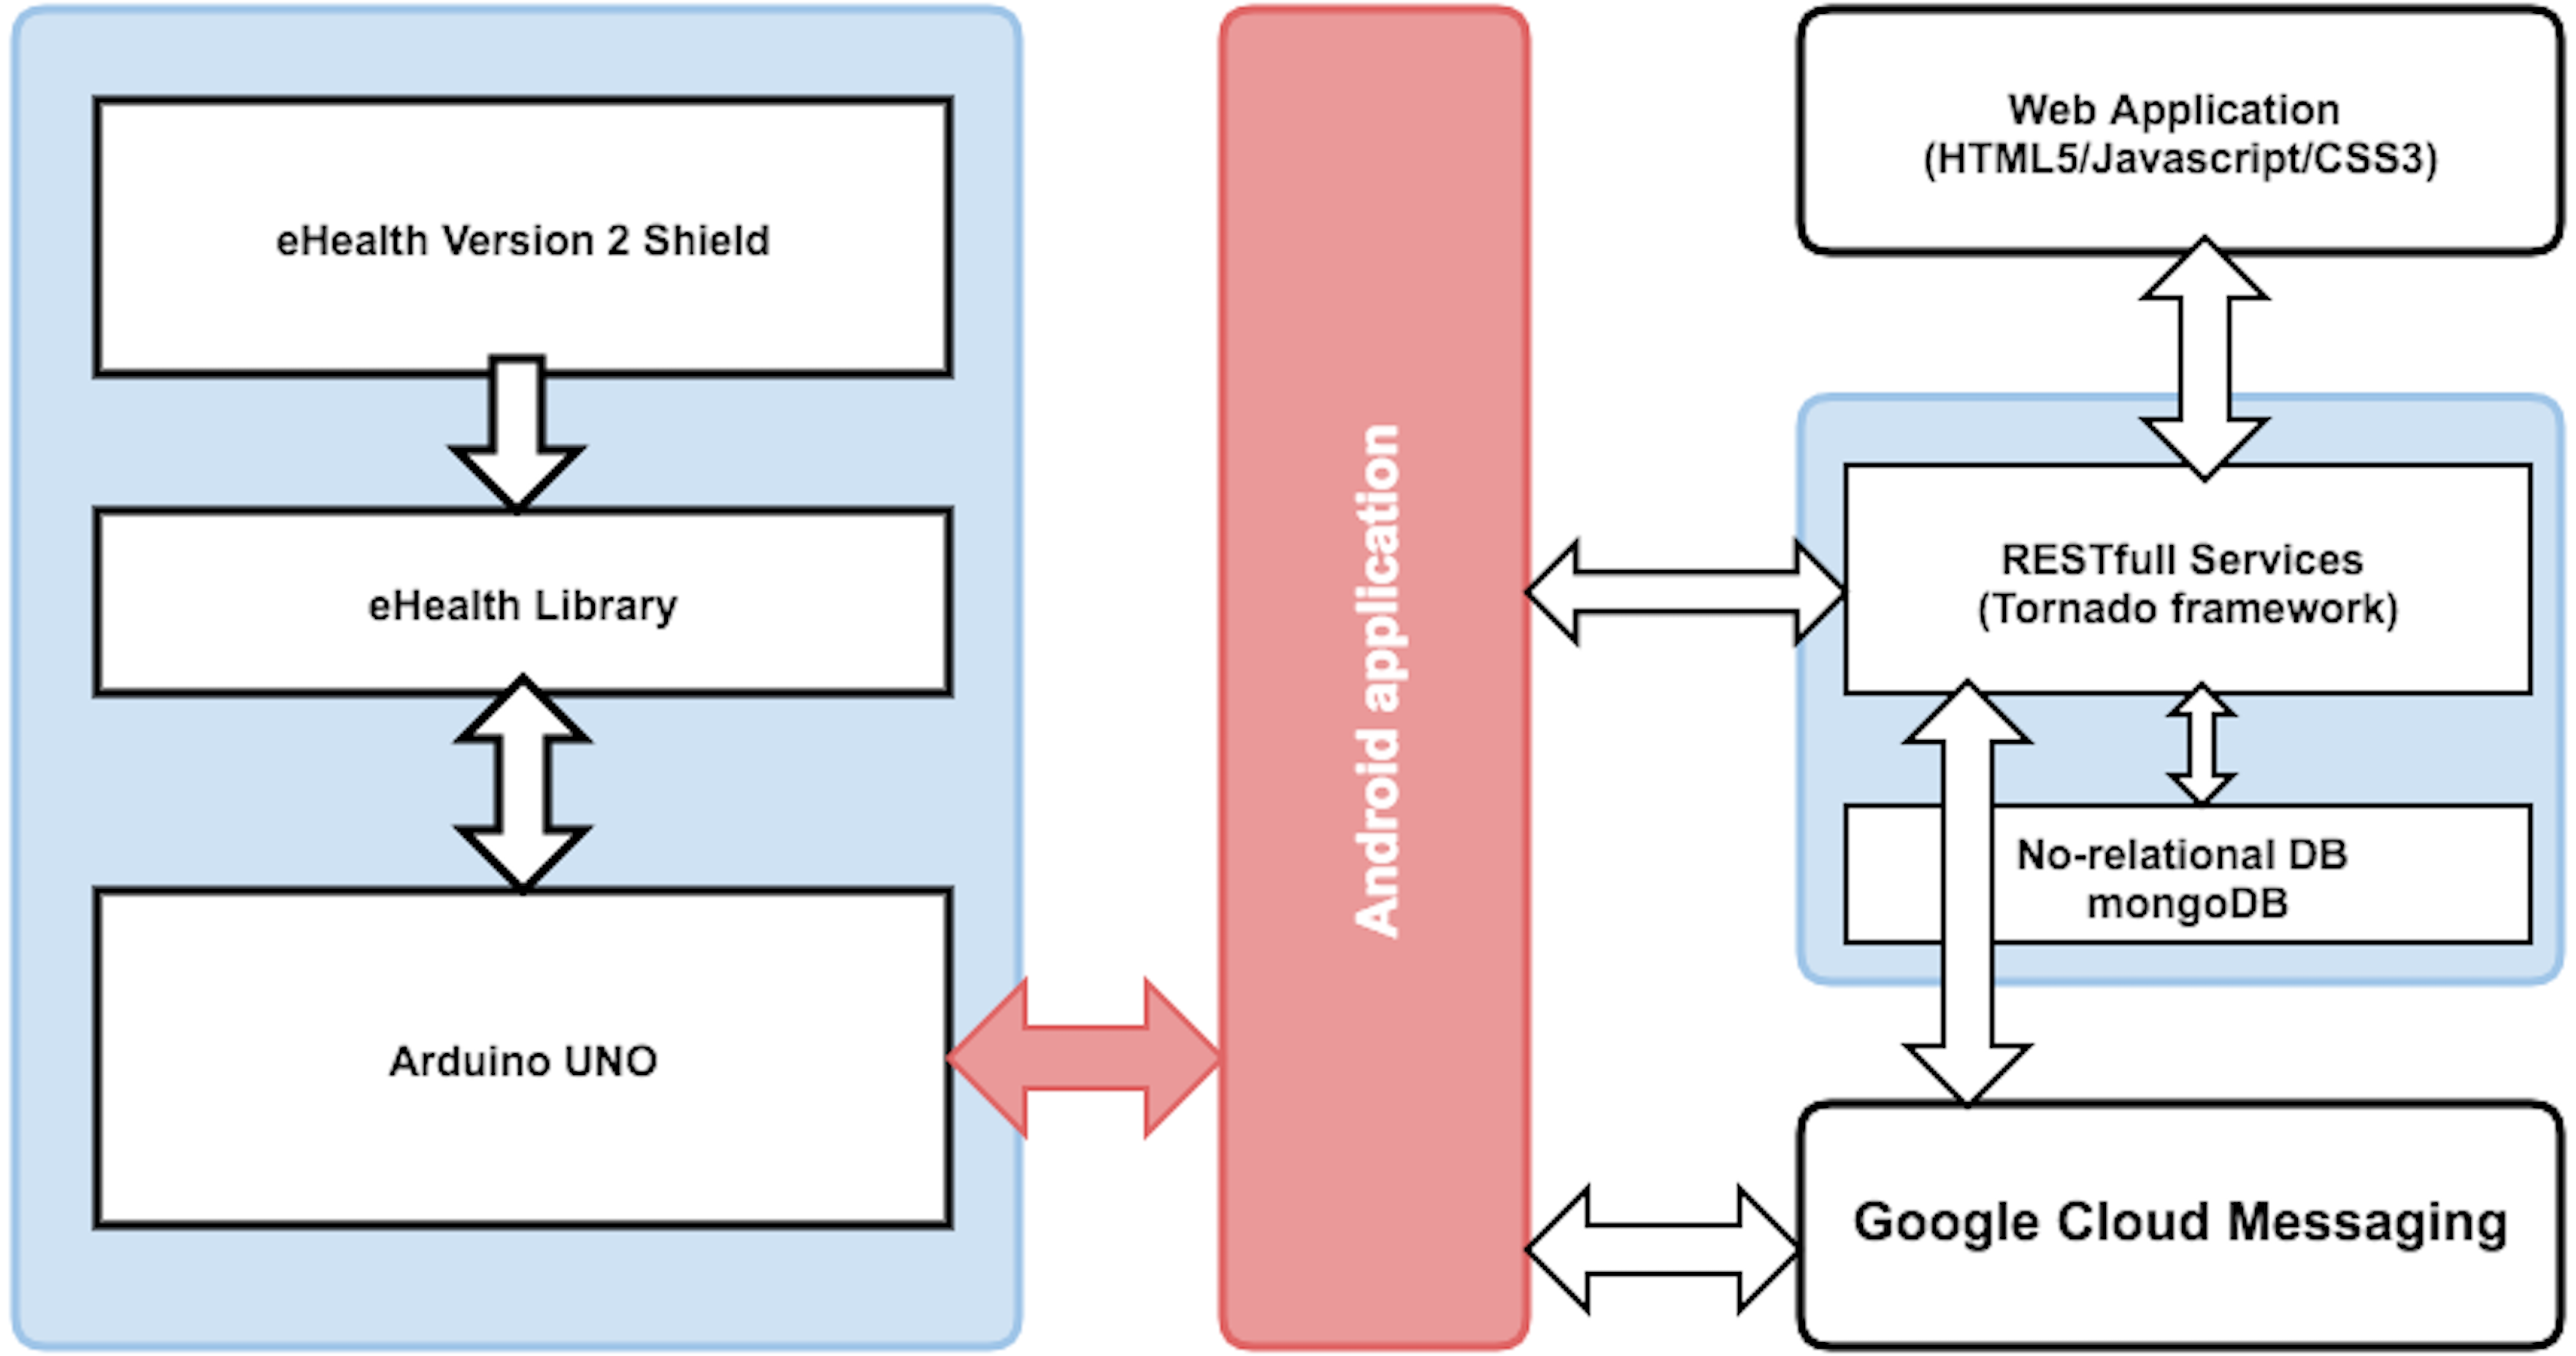
\includegraphics[width=15cm]{images/System_archutecture.png} % This scales the picture to
                                      % a width of 10cm
                                      % You can scale to the
                                      % width or height you need
%\end{center}
\caption{System Architecture}
\label{fig:fig-eg}
\end{figure}

In this work a portable health device is developed for HCWs that can plug into into mobile smartphone device. the concept as it shown in the system architecture figure above is to provide a full stack diagnosing tool based on mobile wireless communication by leveraging already existing technologies. The system is formed by four parts as it is mentioned above. (1) part one with is a health device with three different sensors and responsible of collecting different physiological data. this device consist of an Arduino UNO micro-controller that act as an interface between the device and the second part which is the Android device and application. the communication between the micro-controller and the android device is through USB with the use of build in Android USB HOST Libraries, (2) The android application act as an information display and relay to the third part of the system which act as the base station using mobile wireless technologies. (3) the web application consist of GUI, also this part is responsible of storing data, process and categorize them for better management, (4) the third part is linked to third party communication APIs that allows it to send back instant messages to the mobile device.

\section{Sensors}

As it is mentioned in the system architecture section, the system has three different sensors. Each sensor node measure different type of physiological information. In addition to this three sensors, the Android devices that is used to collect and display the data is also present with different sensors and some of which are used in this works to collect more information about the patients and there environment.
\begin{enumerate}
\item {\bfseries Temperature} Sensor: this sensor is used to measure patient body heat, this sensor can be place to the patient skin such as on the finger or on the leg
\item {\bfseries SPO2 (Peripheral Capillary oxygen saturation ) } sensor: this sensor is responsible of estimating the percentage number of oxygenated hemoglobin compared to the total amount of hemoglobin in the blood
\item {\bfseries ECG (Electro-Cardiogram )} sensor: this sensor is comprised with three electrodes positive, negative and neutral electrodes, that are placed on the patient skin. this sensor is responsible of measuring the electric activities of the patient heart for a certain amount of time
\end{enumerate}

The Sensor devices mentioned above are responsible of monitoring different physiological data of the patient. The table bellow show the specifications of various physiological data that are measured by the sensors.
\begin{table}[H]
\begin{center}
    \begin{tabular}{ |l|l|l| }
\hline
{\bfseries Parameters} & {\bfseries Specifications} \\ \hline
\multirow{5}{*}{Body Temperature} 
  & Hypotermia:  \textless $35$\textdegree C\\
  & Normal      : $36.5$\textdegree C to $37.5$\textdegree C \\
  & Hyperthermia/ Fever: \textgreater $37.5$\textdegree C to $38.3$\textdegree C\\
  & Hyper pyrexia: \textgreater $40.0$\textdegree C to $41.5$ \textdegree C \\ \hline
Oxygen saturation in blood (SaO2) & 0\% to 100\% \\ \hline
\multirow{2}{*}{Electrocardiogram (ECG)} 
 & Frequency: 0.5Hz – 100 Hz  \\
 & Amplitude: 0.25 – 1mV\\
\hline
\end{tabular}
\end{center}
\caption{Various vital parameters measured by the sensors}\label{vital}
\end{table}

\section{Design and Implementation process}


\section{System Requirements}

The designed system is highly described in the above sections of the chapter 4. in this section will try to describe basic requirements for each component of the system to allow the fulfillment of required use case scenarios.

n addition, the system was build around open-source frameworks and eHealth version two kit that was selected to experiment and test out our hypothesis.

\begin{itemize}
\item To allow the CHWs have the tools, in this case sensors and have the applied to patients.
Requirements:
	\begin{enumerate}
		\item eHealth version two kit, This kit must allow all the selected sensors and collect all signals from them
		\item Arduino Uno micro controller, The Arduino should have all the logic and functionality to process the data
		\item eHealth Library software, this library is integrated to allow the eHealth kit to work with Arduino micro controller, in addition this library should facilitate the customization and calibration of sensors
	\end{enumerate}
\item The system should allow the CHWs to visualized the data collect from the sensors and act accordingly. For better decision making the system should also have the capability of sending the data to remote Doctors for further analysis and generate feedbacks to assist CHWs. Requirements:
	\begin{enumerate}
		\item A smart phone device that runs android version 4.0.3 (Ice Cream Sandwich) and higher is required
		\item To connect the Arduino Uno to the smart phone An OTG cable is required for transferring the data from the micro   controller to the smartphone. In addition, this cable will allow the smart phone to power up the micro controller
		\item Google Cloud Messaging (GCM) libraries and configurations, to allow the smart phone to generate alert and notification for The CHWs
	\end{enumerate}
\item A cloud based application (Server Application) should be implemented to store and analyze data for the Doctors to judge and make some form of conclusions. Requirements:
	\begin{enumerate}
		\item RESTFull server with minimum data manipulation web services with some business logic
		\item no-relation database system ( Mongoldb Database) to store the big data generated by the sensors and integrate different resources from different third party APIs
	\end{enumerate}
\end{itemize}

The above requirements are designed to develop a minimum viable product functionality of the prototype. They are also designed to achieve the goal of building a cost effective system that can allow the HCWs to detect and prevent illness at their early stage. Hardware and software details will be discussed in the following points according to the requirements specified in this section. 

\section{System hardware}
\subsection{eHealth version two kit Shield Board}

The eHealth sensor shield platform was developed to be used in the health care sector. the board can be interfaced with different other micro controllers such as Arduino, and a full stack mini computer such as Raspberry Pi. The board was build by cooking hack and can support 10 different health care sensors: body temperature, pulse and Oxygen saturation in blood (SPO2), electrocardiogram (ECG), Airflow sensor, glucometor, galvanic skin response, blood pressure sensor, accelerometer (Patient position) and electromyograph sensor(EMG).
\begin{figure}[H]
\centering
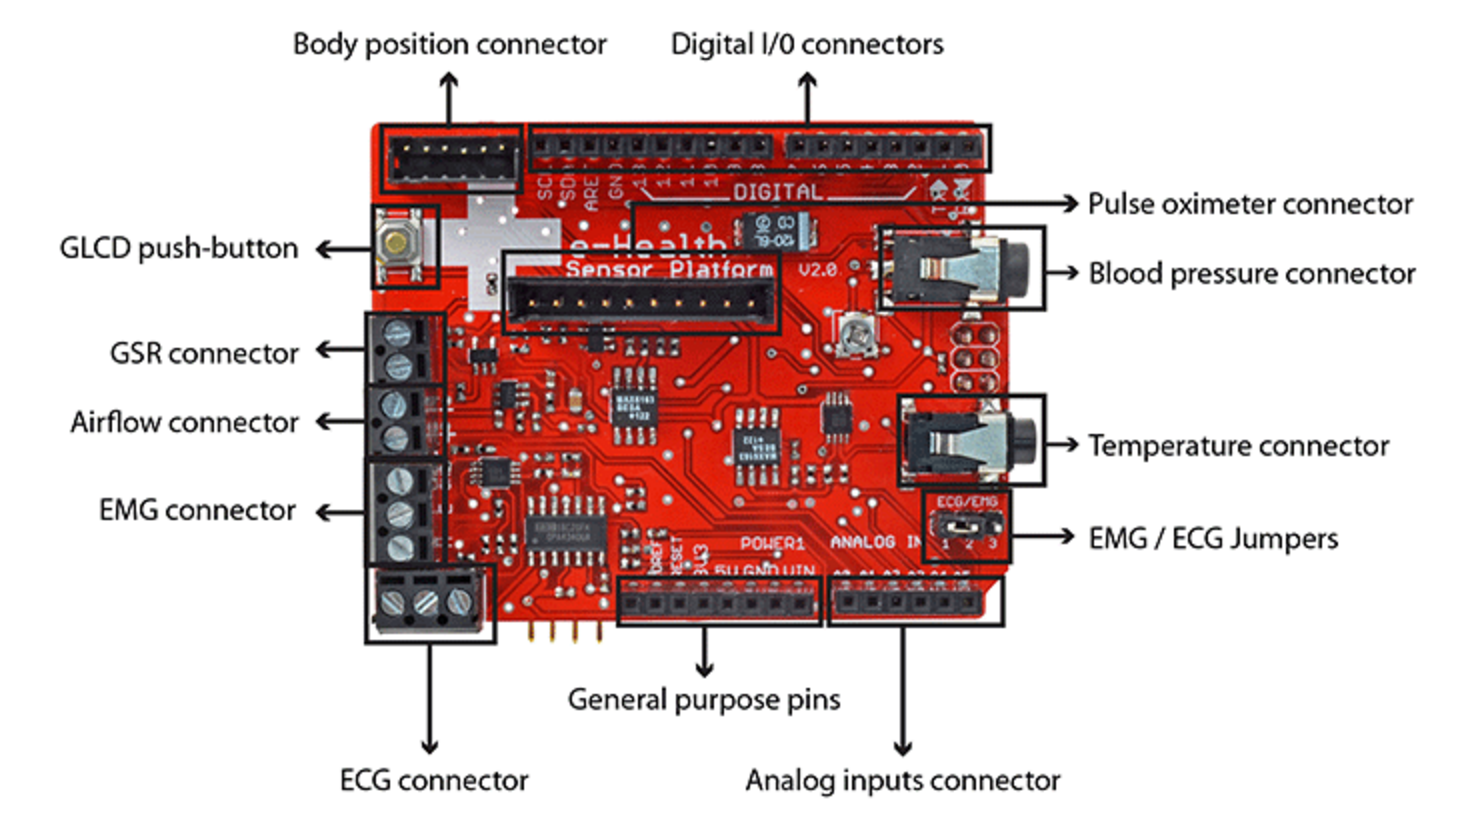
\includegraphics[width=15cm]{images/ehealth_kit.png} % This scales the picture to
                                      % a width of 10cm
                                      % You can scale to the
                                      % width or height you need
%\end{center}
\caption{eHealth sensor shield platform}
\label{fig:fig-eg}
\end{figure}

The board is also capable of supporting a number of communication protocols such as wifi and bluetooth shield board to exchange data with other devices or cloud applications. in this work only three sensors body temperature, ECG and SPO2 sensors were selected to conduct the experiments and implement the prototype.

\subsection{Arduino UNO}

The RDS health device is based on Arduino microprocessor technology. The Arduino is the core part since it is used to collect and process the data from the sensors through the health sensor shield board.

\begin{figure}[H]
\centering
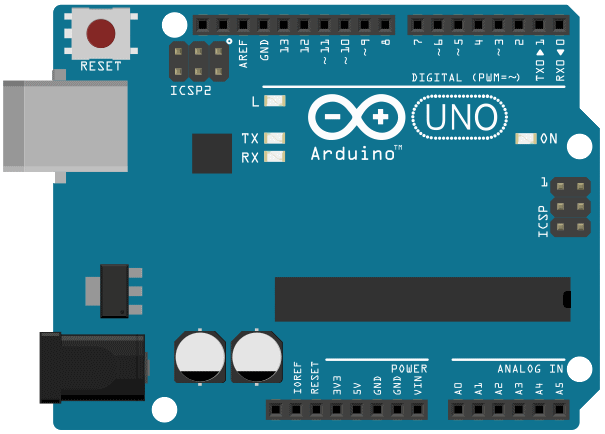
\includegraphics[width=8cm]{images/arduino-uno.png} % This scales the picture to
                                      % a width of 10cm
                                      % You can scale to the
                                      % width or height you need
%\end{center}
\caption{Arduino UNO micro controller board}
\label{fig:fig-eg}
\end{figure}

The figure two above show the Arduino board used in the system. It provides the environment that is easy accessible and compatible to the Android environment. The eHealth shield sensor board shield was build on to work with Arduino board and its health library is easily integrated in the Arduino development environment (IDE). The figure bellow shows the Arduino Uno specification requirements used in the system.

\begin{table}[H]
\begin{center}
    \begin{tabular}{ |l|l|l| }
\hline
{\bfseries Parameters} & {\bfseries Specifications} \\ \hline
Microcontroller & ATmega328P \\ \hline
Operating Voltage & 5V \\ \hline
Input Voltage (recommended) & 7-12V \\ \hline
nput Voltage (limit) & 6-20V \\ \hline
Digital I/O Pins & 14 (of which 6 provide PWM output) \\ \hline
PWM Digital I/O Pins & 6 \\ \hline
Analog Input Pins & 6 \\ \hline
DC Current per I/O Pin & 20 mA \\ \hline
DC Current for 3.3V Pin & 50 mA \\ \hline
\multirow{2}{*}{Flash Memory} 
 & 32 KB (ATmega328P)  \\
 & of which 0.5 KB used by bootloader\\
\hline
SRAM & 2 KB (ATmega328P)\\ \hline
EEPROM & 1 KB (ATmega328P) \\ \hline
Clock Speed & 16 MHz \\ \hline
Lenght & 68.6 mm \\ \hline
Width & 53.4 mm \\ \hline
Weight & 25 g \\ 
\hline

\end{tabular}
\end{center}
\caption{Arduino Microcontroller Technical specification\cite{ArduinoUnoSpecs}}\label{Microcontroller}
\end{table}


\subsection{USB OTG cable }
USB OTG cable is a special USB cable using standards that can allow an android smart phone connect and communicate with peripheral devices. USB OTG (USB On The Go) was developed to give a mobile phone the power to enable other devices, by enabling USB host feature on the android phone. A smart phone with a USB host enabled acts a hub to all connected devices and can be used to addition devices such as keyboards and other devices.

USB OTG cable was used in this work to enable the smart phone as the gateway and can read and process the information from the sensors through the micro controller.

\subsection{Android smart phone}
\subsection{Server hardware}
\section{System Software Design}
